\documentclass[tikz,border=3mm,multi=tikzpicture]{standalone}
\usepackage{tikz}
\usetikzlibrary{arrows.meta,positioning,calc}
\begin{document}

% TikZ 1
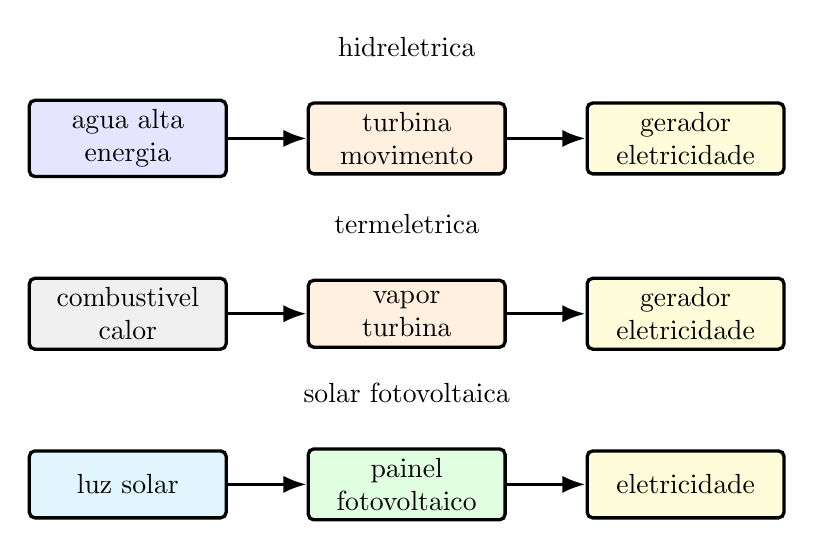
\begin{tikzpicture}[>=Latex,node distance=0.8cm]
  \tikzstyle{box}=[draw,rounded corners=2pt,minimum width=2.5cm,minimum height=0.85cm,align=center,very thick]
  \node[box,fill=blue!10] (agua) {agua alta\\energia};
  \node[box,fill=orange!12,right=1.0cm of agua] (turbina) {turbina\\movimento};
  \node[box,fill=yellow!15,right=1.0cm of turbina] (gerador) {gerador\\eletricidade};
  \draw[very thick,->] (agua) -- (turbina);
  \draw[very thick,->] (turbina) -- (gerador);
  \node[above=0.45cm of turbina] {hidreletrica};

  \node[box,fill=gray!12,below=1.25cm of agua] (comb) {combustivel\\calor};
  \node[box,fill=orange!12,right=1.0cm of comb] (vapor) {vapor\\turbina};
  \node[box,fill=yellow!15,right=1.0cm of vapor] (gerador2) {gerador\\eletricidade};
  \draw[very thick,->] (comb) -- (vapor);
  \draw[very thick,->] (vapor) -- (gerador2);
  \node[above=0.45cm of vapor] {termeletrica};

  \node[box,fill=cyan!12,below=1.25cm of comb] (luz) {luz solar};
  \node[box,fill=green!12,right=1.0cm of luz] (painel) {painel\\fotovoltaico};
  \node[box,fill=yellow!15,right=1.0cm of painel] (ele) {eletricidade};
  \draw[very thick,->] (luz) -- (painel);
  \draw[very thick,->] (painel) -- (ele);
  \node[above=0.45cm of painel] {solar fotovoltaica};
\end{tikzpicture}

% TikZ 2
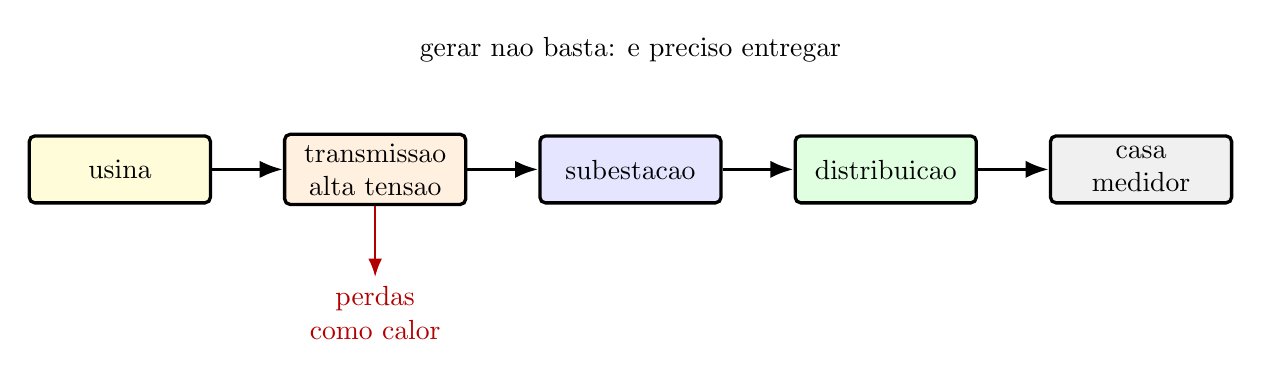
\begin{tikzpicture}[>=Latex,node distance=0.75cm]
  \tikzstyle{box}=[draw,rounded corners=2pt,minimum width=2.3cm,minimum height=0.85cm,align=center,very thick]
  \node[box,fill=yellow!15] (u) {usina};
  \node[box,fill=orange!12,right=0.9cm of u] (t) {transmissao\\alta tensao};
  \node[box,fill=blue!10,right=0.9cm of t] (s) {subestacao};
  \node[box,fill=green!12,right=0.9cm of s] (d) {distribuicao};
  \node[box,fill=gray!12,right=0.9cm of d] (c) {casa\\medidor};
  \draw[very thick,->] (u) -- (t);
  \draw[very thick,->] (t) -- (s);
  \draw[very thick,->] (s) -- (d);
  \draw[very thick,->] (d) -- (c);
  \draw[red!70!black,thick,->] (t.south) -- ++(0,-0.9);
  \node[below,align=center,red!70!black] at ($(t.south)+(0,-0.9)$) {perdas\\como calor};
  \node[align=center,above=0.8cm of s] {gerar nao basta: e preciso entregar};
\end{tikzpicture}

\end{document}
